% Created 2017-02-26 Sun 21:38
% Intended LaTeX compiler: pdflatex
\documentclass[presentation]{beamer}
\usepackage[utf8]{inputenc}
\usepackage[T1]{fontenc}
\usepackage{graphicx}
\usepackage{grffile}
\usepackage{longtable}
\usepackage{wrapfig}
\usepackage{rotating}
\usepackage[normalem]{ulem}
\usepackage{amsmath}
\usepackage{textcomp}
\usepackage{amssymb}
\usepackage{capt-of}
\usepackage{hyperref}
\usetheme{CambridgeUS}
\usecolortheme{beaver}
\setcounter{secnumdepth}{1}
\author{Zheng Tian}
\date{}
\title{Lecture 3: Review of Statistics}
\hypersetup{
 pdfauthor={Zheng Tian},
 pdftitle={Lecture 3: Review of Statistics},
 pdfkeywords={},
 pdfsubject={},
 pdfcreator={Emacs 25.1.1 (Org mode 9.0.3)}, 
 pdflang={English}}
\begin{document}

\maketitle
\begin{frame}{Outline}
\setcounter{tocdepth}{1}
\tableofcontents
\end{frame}



\section{Estimation of the Population Mean}
\label{sec:org5a69501}

\begin{frame}[label={sec:org37a7730}]{The goal of estimation}
\begin{itemize}
\item Suppose we draw \(n\) random samples, \(Y_1, \ldots, Y_n\), and 
\(Y_i \sim IID(\mu_Y, \sigma^2_Y)\) for \(i=1, \ldots, n\).

\item The goal is to estimate \(\mu_Y\) given these \(n\) samples. A natural
way is to compute the sample average, \(\overline{Y}\).
\end{itemize}
\end{frame}

\begin{frame}[label={sec:orgd6b3b12}]{Estimators}
\begin{itemize}
\item An \alert{estimator} is a function of a sample of data to be drawn randomly
from a population.

\item An \alert{estimate} is the numerical value of the
estimator when it is actually computed using data from a specific
sample.

\item An estimator is a random variable because of randomness in
selecting the sample, while an estimate is a nonrandom realization of
the estimator.
\end{itemize}
\end{frame}

\begin{frame}[label={sec:orgb6c0231}]{Estimators of \(\mu_Y\)}
\begin{itemize}
\item \(\overline{Y} = (1/n)\sum_{i=1}^n Y_i\)  is an estimator of
\(\mu_Y\).

\item \(Y_1\), the first observation, can also be used as an
estimator because it is indeed a function of sample data.

\item As such, we can have many different estimators of \(\mu_Y\). How can
we judge which estimator is better than another?
\end{itemize}
\end{frame}

\subsection*{Unbiasedness}
\label{sec:org5dd8e1e}

\begin{frame}[label={sec:orgf76d8ca}]{Definition of unbiased estimators}
\begin{itemize}
\item Let \(\hat{\mu}_Y\) be an estimator of \(\mu_Y\). The estimator
\(\hat{\mu}_Y\) is said to be unbiased if 

\[\mathrm{E}(\hat{\mu}_Y) = \mu_Y\]

where \(\mathrm{E}(\hat{\mu}_Y)\) is the expectation of the
sampling distribution of \(\hat{\mu}_Y\).
\end{itemize}
\end{frame}

\begin{frame}[label={sec:org6f62b91}]{Are \(\overline{Y}\) and \(Y_1\) unbiased?}
\begin{itemize}
\item \(\overline{Y}\) is an unbiased estimator of \(\mu_Y\). 

\vspace{0.3cm}

In Lecture 2, we have already shown that \(\mathrm{E}(\overline{Y}) =
  \mu_Y\) when \(Y_i \sim IID(\mu_Y, \sigma^2_Y)\) for \(i=1, \ldots, n\).

\vspace{0.3cm}

\item \(Y_1\) is also an unbiased estimator. 

\(\mathrm{E}(Y_1) = \mu_Y\) when \(Y_1\) is drawn from \(IID(\mu_Y,
  \sigma^2_Y)\).
\end{itemize}
\end{frame}

\subsection*{Consistency}
\label{sec:orgd175543}

\begin{frame}[label={sec:orgf110a06}]{Definition of consistent estimators}
\begin{itemize}
\item \(\hat \mu_Y\) is a consistent estimator of \(\mu_Y\) if \(\hat{\mu}_Y\)
is convergent in probability to \(\mu_Y\). That is, \(\hat{\mu}_Y\) is
consistent if 

\[\hat{\mu}_Y \xrightarrow{\text{ p }} \mu_Y \text{ as
  } n \rightarrow \infty\]
\end{itemize}
\end{frame}

\begin{frame}[label={sec:orgbb4e617}]{Are \(\overline{Y}\) and \(Y_1\) consistent?}
\begin{itemize}
\item \(\overline{Y}\) is a consistent estimator of \(\mu_Y\). 

\vspace{0.3cm}

The law of large number ensures that \(\overline{Y}
  \xrightarrow{\text{ p }} \mu_Y\) is true when \(Y_i \sim IID(\mu_Y,
  \sigma^2_Y)\) for \(i=1, \ldots, n\), and \(\sigma^2_Y < \infty\).

\vspace{0.3cm}

\item However, we cannot assess the consistency for \(Y_1\) because it cannot
be written as the form of an average.
\end{itemize}
\end{frame}

\subsection*{Variance and efficiency}
\label{sec:orgad5767a}

\begin{frame}[label={sec:org040d5e9}]{Definition of efficient estimators}
\begin{itemize}
\item When both \(\tilde{\mu}_Y\) and \(\hat{\mu}_Y\) are two unbiased
estimators of \(\mu_Y\), we choose the estimator with the tightest
sampling distribution, which means the smallest variance.

\item \(\hat{\mu}_Y\) is said to be more efficient than \(\tilde{\mu}_Y\) if
\[\mathrm{Var}(\hat{\mu}_Y) < \mathrm{Var}(\tilde{\mu}_Y)\]

\item In words, \(\hat{\mu}_Y\) is more efficient than \(\tilde{\mu}_Y\)
because \(\hat{\mu}_Y\) uses the information in the data more
efficiently than does \(\tilde{\mu}_Y\).
\end{itemize}
\end{frame}

\begin{frame}[label={sec:org7c03ab8}]{\(\overline{Y}\) is more efficient than \(Y_1\)?}
\begin{itemize}
\item In Lecture 2, we compute the variance of \(\overline{Y}\) to be
\(\sigma^2_Y / n\) when \(Y_i \sim IID(\mu_Y, \sigma^2_Y)\).

\item The variance of \(Y_1\) is \(\sigma^2_Y\).

\item When \(n > 1\), \(\overline{Y}\) is more
efficient than \(Y_1\).
\end{itemize}
\end{frame}

\subsection*{\(\overline{Y}\) is the best linear unbiased estimator (BLUE)}
\label{sec:org58466c3}

\begin{frame}[label={sec:org6f6a6c5}]{BLUE}
\begin{itemize}
\item \(\overline{Y}\) happens to be the \alert{Best Linear Unbiased Estimator
(BLUE)}.

\item It means that among all linear unbiased estimator,
\(\overline{Y}\) has the smallest variance.
\end{itemize}
\end{frame}

\begin{frame}[label={sec:orgd0079d4}]{Linear estimators and \(\overline{Y}\) is BLUE}
\begin{itemize}
\item A linear estimator of \(\mu_Y\) is a weighted average of \(Y_1, \ldots,
  Y_n\), written as
\[ \tilde{\mu}_Y = \frac{1}{n} \sum_{i=1}^n \alpha_i Y_i \]
where \(\alpha_1, \ldots, \alpha_n\) are nonrandom constants.

\item If \(\tilde{\mu}_Y\) is another unbiased estimator of \(\mu_Y\),
then we always have \(\mathrm{Var}(\overline{Y}) \leq
  \mathrm{Var}(\tilde{\mu}_Y)\), and the equality holds only if
\(\tilde{\mu}_Y = \overline{Y}\). It means that \(\overline{Y}\) is BLUE.
\end{itemize}
\end{frame}

\subsection*{\(\overline{Y}\) is the least squares estimator of \(\mu_Y\)}
\label{sec:org09cc3db}

\begin{frame}[label={sec:org3ab671d}]{A linear model for the population mean}
\begin{itemize}
\item Consider the following model
\[ Y_i = \alpha + u_i \text{ for } i = 1, 2, \ldots, n \]
where \(\alpha\) is a nonrandom intercept to be estimated.

\item \(u_i\) is the error term, which is a random variable with
\(\mathrm{E}(u_i) = 0\).  Thus, we have \(E(Y_i) = \alpha = \mu_Y\).

\item \(u_i\) can be seen as the error of predicting \(Y_i\) with \(\alpha\) for
each \(i\), and we use 
\[\sum_{i=1}^n (Y_i - \alpha)^2\] 
to measure the total prediction errors.

\item A natural choice of an estimator of \(\alpha\) is the one that
minimizes this sum of squared errors.
\end{itemize}
\end{frame}

\begin{frame}[label={sec:org7d074b1}]{The least squares estimator}
\begin{itemize}
\item The least squares estimator of \(\mu_Y\) (or \(\alpha\)) is obtained by
solving the following problem
\[ \operatorname*{min}_a\: \sum_{i=1}^n (Y_i - a)^2 \]

\item The solution of this minimization problem is just \(a = \overline{Y}\).
\end{itemize}
\end{frame}

\begin{frame}[label={sec:org93bc69a}]{The proof for \(\overline{Y}\) is the least square estimator}
\begin{itemize}
\item The first order condition for the minimization problem is

\begin{equation*}
  \frac{d}{da}\sum_{i=1}^n (Y_i - a)^2 = -2\sum_{i=1}^n(Y_i - a) = -2\sum_{i=1}^n Y_i+ 2n a = 0      
\end{equation*}

\item Solving the equation for \(a\), we get \(a = 1/n\sum_{i=1}^n Y_i = \overline{Y}\).
\end{itemize}
\end{frame}


\section{Hypothesis Tests Concerning the Population Mean}
\label{sec:orgea55d7e}

\begin{frame}[label={sec:orge000b81}]{The null hypothesis}
\begin{itemize}
\item Hypothesis testing is thus to make a provisional
decision based on the evidence at hand on.

\item The hypothesis of the population mean, \(\mathrm{E}(Y)\), taking on a
specific value, \(\mu_{Y,0}\). So the null hypothesis, denoted as
\(H_0\), is 
 \[ H_0: E(Y) = \mu_{Y,0} \]
\end{itemize}
\end{frame}

\begin{frame}[label={sec:org5b3f53b}]{The alternative hypothesis}
\begin{itemize}
\item The alternative hypothesis, denoted as \(H_1\)
\begin{itemize}
\item The two-sided alternative: \(H_1: E(Y) \neq \mu_{Y,0}\)
\item The one-sided alternative: \(H_1: E(Y) > \mu_{Y,0}\)
\end{itemize}

\item The language 

One thing should be kept in mind is that we usually do not say "accept
the null hypothesis" when the hypothesis test is in favor of the null,
but say "fail to reject the null".
\end{itemize}
\end{frame}

\begin{frame}[label={sec:orgbfb1c4a}]{The z-statistic when \(\sigma_Y\) is known}
\begin{itemize}
\item We know that when \(Y_i \sim IID(\mu_Y, \sigma^2_Y)\) for \(i=1, \ldots,
  n\), \(E(\overline{Y}) = \mu_Y\) and
\(\mathrm{Var}(\overline{Y}) = \sigma^2_{\overline{Y}} = \sigma^2_Y /
  n\).

\item In the null hypothesis, we specify \(\mu_Y = \mu_{Y,0}\).

\item So given that \(\sigma_Y\) is known, the z-statistic is computed as 

\[ z = \frac{\overline{Y} -
  \mu_{Y,0}}{\sigma_{\overline{Y}}} = \frac{\overline{Y} -
  \mu_{Y,0}}{\sigma_Y/\sqrt{n}} \]

\item As \(n \rightarrow \infty\), by the central limit theorem, we know \(z
  \xrightarrow{\text{ d }} N(0, 1)\).
\end{itemize}
\end{frame}

\begin{frame}[label={sec:orgbb1706d}]{The t-statistic when \(\sigma_Y\) is unknown}
\begin{itemize}
\item Of course, \(\sigma_Y\) is the standard deviation of the population
variance that is usually unknown. So we need to replace \(\sigma_Y\)
with its estimator.
\end{itemize}
\end{frame}

\begin{frame}[label={sec:org08ec69b}]{The sample variance and standard deviation}
\begin{itemize}
\item The \alert{sample variance} \(s^2_Y\) is is an estimator of the population
variance \(\sigma^2_Y\), which is computed as

\[ s^2_Y = \frac{1}{n-1}\sum^n_{i=1} (Y_i - \overline{Y})^2 \]

\item The \alert{sample standard deviation}, \(s_Y\), is the square root of \(s^2_Y\)

\item The sample variance, \(s^2_Y\), is a consistent estimator of the
population variance, that is, as 

\[ n \rightarrow \infty, s^2_Y \xrightarrow{\text{ p }} \sigma^2_Y\]
\end{itemize}
\end{frame}

\begin{frame}[label={sec:orgd86593a}]{The standard error of \(\overline{Y}\)}
\begin{itemize}
\item The standard error of \(\overline{Y}\), denoted as \(SE(\overline{Y})\) or
\(\hat{\sigma}_{\overline{Y}}\), is an estimator of the standard
deviation of \(\overline{Y}\), \(\sigma_{\overline{Y}}=\sigma_Y/\sqrt{n}\), with \(s_Y\) replacing
\(\sigma_Y\). 

\[ SE(\overline{Y}) = \hat{\sigma}_{\overline{Y}} =
  \frac{s_Y}{\sqrt{n}} \]
\end{itemize}
\end{frame}

\begin{frame}[label={sec:orgd2105ae}]{The t-statistic}
\begin{itemize}
\item When \(\sigma_Y\) is unknown, by replacing \(\sigma_Y\) with \(s_Y\), we
have the t statistic
\end{itemize}

\[ t = \frac{\overline{Y} - \mu_{Y,0}}{SE(\overline{Y})} =
  \frac{\overline{Y} - \mu_{Y,0}}{s_Y/\sqrt{n}} \] 

\begin{itemize}
\item The asymptotic distribution of the t statistic is \(N(0, 1)\) because
\(s_Y\) is a consistent estimator of \(\sigma_Y\).

\item When \(Y_i\) for \(i=1, \ldots, n\) are i.i.d. from \(N(\mu_Y,
  \sigma_Y^{2})\), we can show that the exact distribution for the t
statistic is the student t distribution with \((n-1)\) degrees of
freedom. That is
\[ t \sim t(n-1)  \]
\end{itemize}
\end{frame}

\begin{frame}[label={sec:org2a4cd8c}]{Hypothesis testing with a pre-specified significance level}
With the null and alternative hypotheses being the goal of the test
and test statistics being the tools, we need a rule to make a
judgment: When can we reject (or fail to reject) the null hypothesis
if the test statistic takes on what values? To do so, we need to first
define some concepts. 
\end{frame}


\begin{frame}[label={sec:org1e61630}]{Type I and type II errors}
\begin{itemize}
\item A statistical hypothesis test can make two types of mistakes:
\begin{itemize}
\item \alert{Type I error}. The null hypothesis is rejected when in fact it is
true.
\item \alert{Type II error}. The null hypothesis is not rejected when in fact it
is false.
\end{itemize}
\end{itemize}
\end{frame}

\begin{frame}[label={sec:orge57aae4}]{The significance level and the critical value}
\begin{itemize}
\item The \alert{significance level} is the pre-specified probability of type I error.
Usually, we set the significance level to be \(\alpha = 0.05, 0.10,
  \text{ or } 0.01\).

\item The \alert{critical value}, denoted as \(c_{\alpha}\), is the value of the
test statistic for which the test rejects the null hypothesis at the
given significance level. The \(N(0, 1)\) critical value for a
two-sided test with a 5\% significance level is 1.96.
\end{itemize}
\end{frame}

\begin{frame}[label={sec:org0275c53}]{The rejection rule and rejection region}
\begin{itemize}
\item The \alert{rejection rule}. For a two-sided test, we reject the null
hypothesis when \(|z^{act}| > c_{\alpha}\).

\item The \alert{rejection region} is the set of values of the test statistic
for which the test rejects the null, and the \alert{acceptance region} is
the vice.
\end{itemize}
\end{frame}

\begin{frame}[label={sec:org8133735}]{The rejection region illustrated}
\begin{figure}[htbp]
\centering
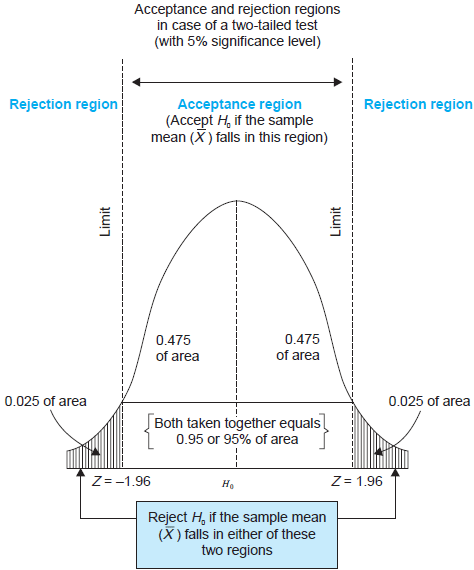
\includegraphics[width=0.5\textwidth]{figure/fig9_1.png}
\caption{\label{fig:org6702ca2}
An illustration of a two-sided test}
\end{figure}
\end{frame}

\begin{frame}[label={sec:org277777d}]{The power and the size of the test}
\begin{itemize}
\item The \alert{size} of the test is the probability that the test actually
incorrectly rejects the null hypothesis when it is true. That is,
the size of the test is just the significance level.

\item The \alert{power} of the test is the probability that the test correctly
rejects the null when the alternative is true. That is,

\[\text{power} = 1 - \mathrm{Pr}(\text{type II error})\]
\end{itemize}
\end{frame}

\begin{frame}[label={sec:orgb7e3fd2}]{The p-value}
\begin{itemize}
\item The \alert{p-value}, also called the \alert{significance probability}, is the
probability of drawing a statistic at least as adverse to the null
hypothesis as the one you actually computed in your sample, assuming
the null hypothesis is correct.

\item The p-value provides more information than the significance level. 

In fact, the p-value is also named the marginal significance level,
which the smallest significance level at which you can reject the
null hypothesis.
\end{itemize}
\end{frame}

\begin{frame}[label={sec:org7169bf1}]{Rejection rule with the p-value}
\begin{itemize}
\item The rejection rule of rejecting the null is then
the \(\text{p-value} < \alpha\).

\item Mathematically, the p-value is computed as

\begin{equation*}
p\text{-value} = 
\begin{cases}
\mathrm{Pr}_{H_0}\left(|z| > |z^{act}|\right)=2\Phi(-|z^{act}|) \text{ when } \sigma_Y \text{ is known} \\
\mathrm{Pr}_{H_0}\left(|t| > |t^{act}|\right)=2\Phi(-|t^{act}|) \text{ when } \sigma_Y \text{ is unknown}
\end{cases}
\end{equation*}
\end{itemize}
\end{frame}

\begin{frame}[label={sec:org4ab8b28}]{One-sided alternatives}
\begin{itemize}
\item For a one-sided alternative hypothesis, \(H_1: \mathrm{E}(Y) >
  \mu_{Y,0}\), we can compute the p-value as
\[ p\text{-value} = \mathrm{Pr}_{H_0}(t > t^{act}) = 1 - \Phi(t^{act}) \]

\item The \(N(0, 1)\) critical value for a one-sided test with a 5\%
significance level is 1.64. The rejection region for this test is all
values of the t-statistic exceeding 1.64.
\end{itemize}
\end{frame}


\section{Confidence Intervals for the Population Mean}
\label{sec:orgeeb49e9}

\begin{frame}[label={sec:org033d5f4}]{Definitions}
\begin{itemize}
\item A \alert{confidence set} is the set of values that contains the true
population mean \(\mu_Y\) with a certain prespecified probability.

\item A \alert{confidence level} is the prespecified probability that \(\mu_Y\) is
contained in the confidence set. \(\text{confidence level} = 1 -
  \text{significance level}\).

\item A \alert{confidence interval} is the confidence set when it is an
interval.

\item In the case of a two-sided test for \(\mu_Y\), we say that a 95\%
confidence interval is an interval constructed so that it contains
the true value of \(\mu_Y\) in 95\% of all possible random samples.
\end{itemize}
\end{frame}

\begin{frame}[label={sec:orgd349ed7}]{Constructing a confidence interval based on the t statistic}
\begin{itemize}
\item Step 1: we compute the t statistic for the two-sided test
\[ t = \frac{\overline{Y} - \mu_{Y,0}}{SE(\overline{Y})}
   \xrightarrow{\text{ d }} N(0, 1) \]

\item Step 2: we know that we fail to reject the null at the 5\% level if \(|t| <
  1.96\).

\item Step 3: we plug in the definition of \(t\) and solving for \(|t| \leq 1.96\), we
get
\begin{align*}
-1.96 & \leq \frac{\overline{Y} - \mu_{Y,0}}{SE(\overline{Y})} \leq 1.96 \\
\overline{Y} - 1.96 SE(\overline{Y}) & \leq \mu_{Y,0} \leq \overline{Y} + 1.96 SE(\overline{Y})
\end{align*}
\end{itemize}
\end{frame}

\begin{frame}[label={sec:orgc9c6854}]{The 95\%, 90\%, and 99\% confidence interval}
\begin{itemize}
\item The 95\% confidence interval two-sided confidence interval for
\(\mu_Y\) is 
\[ \{ \overline{Y} \pm 1.96 SE(\overline{Y}) \} \]
\item 90\% confidence interval for \(\mu_Y = \{ \overline{Y} \pm 1.64
  SE(\overline{Y}) \}\)
\item 99\% confidence interval for \(\mu_Y = \{ \overline{Y} \pm 2.58
  SE(\overline{Y}) \}\)
\end{itemize}
\end{frame}


\section{Comparing Means from Different Populations}
\label{sec:org45a98f3}

\begin{frame}[label={sec:orga4d4622}]{Hypothesis tests for the difference between two means}
\begin{itemize}
\item The question is whether there is a difference
in earnings between male college graduates and female college
graduates.

\item Let \(Y_{m, i}\) for \(i=1, \ldots, n_m\) be \(n_m\) i.i.d. samples from the
population of earnings of male college graduate, i.e., 

\[ Y_{m,i} \sim IID(\mu_m, \sigma^2_m)  \text{ for } i=1,\ldots,n_m \]

\item Let \(Y_{w, j}\) for \(j=1, \ldots, n_w\) be \(n_w\) i.i.d. samples from
the population of earnings of female college graduate, i.e.,

\[ Y_{w,j} \sim IID(\mu_w, \sigma^2_w)  \text{ for } j=1,\ldots,n_w \]

\item Also, we assume that \(Y_{m,i}\) and \(Y_{w,j}\) are independent.
\end{itemize}
\end{frame}

\begin{frame}[label={sec:org17000cd}]{The null and alternative hypotheses}
\begin{itemize}
\item The hypothesis to be tested is whether the mean earnings for the male and
female graduates differ by a certain amount, that is, 

\[ H_0: \mu_m - \mu_w = d_0,\; \text{ vs. }\: H_1: \mu_m - \mu_w \neq d_0 \]
\end{itemize}
\end{frame}

\begin{frame}[label={sec:org861ab74}]{The test procedures: step 1}
\begin{itemize}
\item Calculate the sample average earnings:

\begin{itemize}
\item \(\overline{Y}_m\) for the
male and \(\overline{Y}_w\) for the female.

\item As \(n_m\) and \(n_w\) get large, we know \(\overline{Y}_m
    \xrightarrow{\text{ d }} N(\mu_Y, \sigma^2_m/n_m)\), and
\(\overline{Y}_w \xrightarrow{d} N(\mu_w, \sigma^2_w / n_w)\).

\item Given that \(\overline{Y}_m - \overline{Y}_w\) is a linear function
of \(\overline{Y}_m\) and \(\overline{Y}_w\), and \(Y_{m,i}\) and
\(Y_{w,j}\) are independent, we know that 
\[(\overline{Y}_m - \overline{Y}_w) \xrightarrow{d} N(\mu_m -
    \mu_w,\; \frac{\sigma^2_m}{n_m} + \frac{\sigma^2_w}{n_w}) \]
\end{itemize}
\end{itemize}
\end{frame}

\begin{frame}[shrink,label={sec:orgc9d4c81}]{Step 2}
\begin{itemize}
\item When \(\sigma^2_m\) and \(\sigma^2_w\) are known, we use the z statistic
\[ z = \frac{(\overline{Y}_m - \overline{Y}_w) - d_0}{\left(
  \frac{\sigma^2_m}{n_m} + \frac{\sigma^2_w}{n_w} \right)^{1/2}}
  \xrightarrow{\text{ d }} N(0, 1) \]

\item When \(\sigma^2_m\) and \(\sigma^2_w\) are unknown, we the t
statistic
\[ t = \frac{(\overline{Y}_m - \overline{Y}_w) -
  d_0}{SE(\overline{Y}_m - \overline{Y}_w)} \xrightarrow{d}
  N(0, 1) \] 
where
\begin{gather*}
SE(\overline{Y}_m - \overline{Y}_w) = \left(\frac{s^2_m}{n_m} + \frac{s^2_w}{n_w} \right)^{1/2} \\
s^2_m = \frac{1}{n_m-1}\sum^{n_m}_{i=1}(Y_{m,i} - \overline{Y}_m)^2 \\
s^2_w = \frac{1}{n_w-1}\sum^{n_w}_{i=1}(Y_{w,i} - \overline{Y}_w)^2
\end{gather*}
\end{itemize}
\end{frame}

\begin{frame}[label={sec:org4343fb2}]{Step 3}
\begin{itemize}
\item Calculate the p value: The p value for the two-sided test is calculated as 

\[ p\text{-value} = 2\Phi(-|t|) \]

\item For a two-sided test at the 5\% significant level, we can reject
the null hypothesis when the p value is less than 5\%, or,
equivalently, when \(|t| > 1.96\).
\end{itemize}
\end{frame}

\begin{frame}[label={sec:orge545ba2}]{Confidence intervals for the difference between two means}
\begin{itemize}
\item The 95\% confidence interval can be constructed as usual based on the t
statistic we have computed above.

\item The 95\% confidence interval for \(d = \mu_m - \mu_w\) is

\[ (\overline{Y}_m - \overline{Y}_w) \pm 1.96SE(\overline{Y}_m -
  \overline{Y}_w) \]
\end{itemize}
\end{frame}

\begin{frame}[label={sec:org9fdc757}]{Differences-of-Means Estimation of Causal Effects Using Experimental Data}
\begin{itemize}
\item We define the outcome of a randomized controlled experiment to be \(Y\)
and the binary treatment variable to be \(X\), \(X=1\) for the treatment
group and \(X=0\) for the control group.

\item Then the causal effect of the
treatment can be conveniently expressed as the difference in the
conditional expectation
\[ E(Y \mid X=1) - E(Y \mid X=0) \]
\end{itemize}
\end{frame}


\section{Scatterplots, the Sample Covariance, and the Sample Correlation}
\label{sec:orgc51d2b2}

\begin{frame}[label={sec:org245a63a}]{Scatterplots}
\begin{itemize}
\item Exploratory data analysis. Drawing graphs is an important aspect of exploratory data
analysis to visualize the patterns of the variables of
interests.

\item A \alert{scatterplot} is a plot of \(n\) observations on \(X_i\) and \(Y_i\), in
which each observation is represented by the point \((X_i,
  Y_i)\)
\end{itemize}
\end{frame}

\begin{frame}[label={sec:org1bc25ab}]{An example of scatterplot}
\begin{figure}[htbp]
\centering
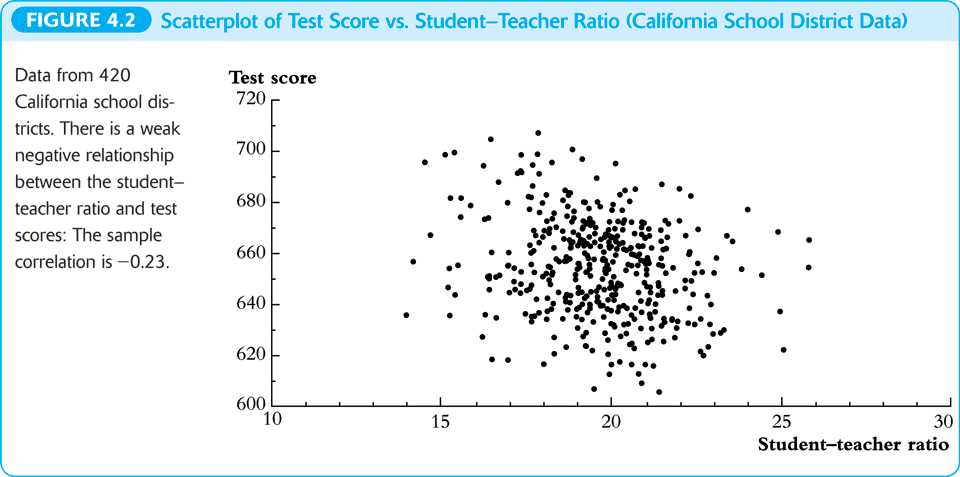
\includegraphics[width=0.9\textwidth]{figure/fig-4-2.png}
\caption{\label{fig:org85ab4e9}
The scatterplot between test scores and student-teacher ratios}
\end{figure}
\end{frame}

\begin{frame}[label={sec:org45e8dc1}]{Sample covariance and sample correlation coefficient}
\begin{itemize}
\item The \alert{sample covariance}, denoted as \(s_{XY}\), is
\[ s_{XY} = \frac{1}{n-1}\sum^n_{i=1}(X_i - \overline{X})(Y_i -
  \overline{Y}) \]

\item The \alert{sample correlation coefficient}, denoted as \(r_{XY}\), is
\[ r_{XY} = \frac{s_{XY}}{s_X s_Y} \]
and we have \(|r_{XY}| \leq 1\).

\item If \((X_i,\, Y_i)\) are i.i.d. and \(X_i\) and \(Y_i\) have finite fourth
moments, then
\[ s_{XY} \xrightarrow{\text{ p }} \sigma_{XY} \text{ and } r_{XY}
  \xrightarrow{\text{ p } } \rho_{XY} \]
\end{itemize}
\end{frame}

\begin{frame}[label={sec:org1c71f65}]{The correlation coefficient measures the linear association}
We should emphasize that the correlation coefficient is a measure of
linear association between \(X\) and \(Y\).

\begin{figure}[htbp]
\centering
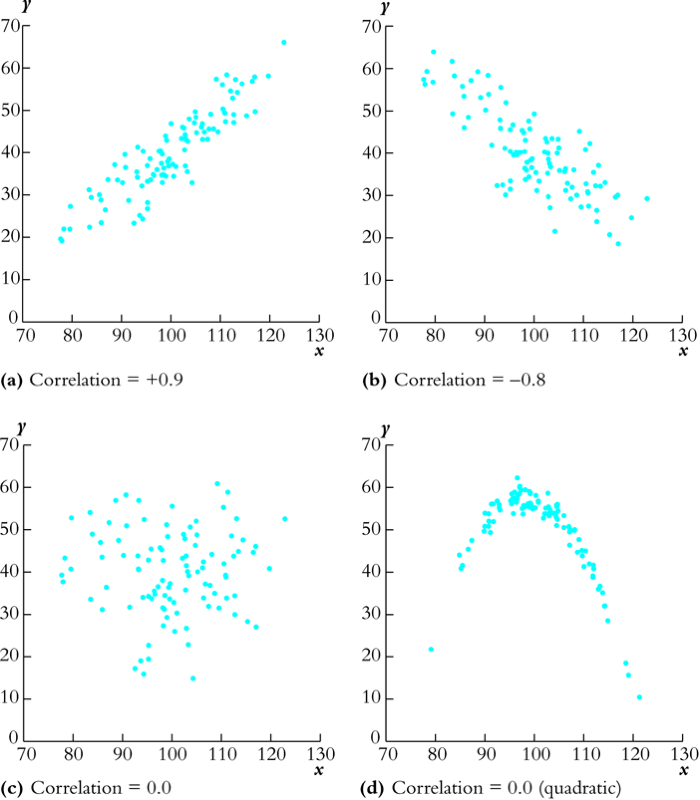
\includegraphics[width=0.5\textwidth]{figure/fig-3-3.png}
\caption{\label{fig:orgea3eaa0}
Scatterplots for four hypothetical data sets}
\end{figure}
\end{frame}
\end{document}